% ═══════════════════════════════════════════════════════════════════════════════
% OpenMagnetics Professional Power Transformer Datasheet
% ═══════════════════════════════════════════════════════════════════════════════
% Industry-standard format for flyback transformers, forward converters, etc.
% Compatible with LatexReportGenerator template tag replacement
%
% Version: 2.0
% ═══════════════════════════════════════════════════════════════════════════════

\documentclass[10pt,a4paper]{article}

% ═══════════════════════════════════════════════════════════════════════════════
% PACKAGES
% ═══════════════════════════════════════════════════════════════════════════════
\usepackage[utf8]{inputenc}
\usepackage[T1]{fontenc}
\usepackage{helvet}
\renewcommand{\familydefault}{\sfdefault}
\usepackage{geometry}
\usepackage{graphicx}
\usepackage{booktabs}
\usepackage{xcolor}
\usepackage{array}
\usepackage{fancyhdr}
\usepackage{tikz}
\usepackage{colortbl}
\usepackage{multirow}
\usepackage{tabularx}
\usepackage{float}
\usepackage{siunitx}
\usepackage{hyperref}
\usepackage{enumitem}
\usepackage{tcolorbox}
\usepackage{calc}
\usepackage{circuitikz}

\usetikzlibrary{shapes,arrows,positioning,calc}

% ═══════════════════════════════════════════════════════════════════════════════
% DOCUMENT SETUP
% ═══════════════════════════════════════════════════════════════════════════════
\geometry{left=12mm, right=12mm, top=15mm, bottom=15mm}
\setlength{\parindent}{0pt}
\setlength{\parskip}{0pt}

% Color definitions
\definecolor{primary}{RGB}{102, 51, 153}      % Purple for transformers
\definecolor{secondary}{RGB}{138, 43, 226}    % Violet accent
\definecolor{accent}{RGB}{255, 140, 0}        % Orange for highlights
\definecolor{lightbg}{RGB}{250, 245, 255}     % Light purple background
\definecolor{gridbg}{RGB}{245, 240, 250}      % Alternating row color
\definecolor{textdark}{RGB}{33, 37, 41}
\definecolor{textmuted}{RGB}{108, 117, 125}
\definecolor{success}{RGB}{40, 167, 69}
\definecolor{warning}{RGB}{255, 193, 7}
\definecolor{danger}{RGB}{220, 53, 69}

% ═══════════════════════════════════════════════════════════════════════════════
% HEADER AND FOOTER
% ═══════════════════════════════════════════════════════════════════════════════
\pagestyle{fancy}
\fancyhf{}
\fancyhead[L]{\footnotesize\color{textmuted}{{COMPANY_NAME}}}
\fancyhead[C]{\footnotesize\textbf{\color{primary}{{PART_NUMBER}}} - Power Transformer}
\fancyhead[R]{\footnotesize\color{textmuted}Rev. {{REVISION}}}
\fancyfoot[L]{\footnotesize\color{textmuted}Generated by OpenMagnetics}
\fancyfoot[C]{\footnotesize\color{textmuted}\thepage\ of \pageref{LastPage}}
\fancyfoot[R]{\footnotesize\color{textmuted}\today}
\renewcommand{\headrulewidth}{0.4pt}
\renewcommand{\footrulewidth}{0.4pt}

% ═══════════════════════════════════════════════════════════════════════════════
% CUSTOM COMMANDS
% ═══════════════════════════════════════════════════════════════════════════════
\newcommand{\sectiontitle}[1]{%
    \vspace{3mm}%
    {\large\bfseries\color{primary}#1}%
    \vspace{1mm}%
    \hrule height 0.3pt%
    \vspace{2mm}%
}

\newcommand{\specvalue}[1]{\textbf{#1}}

\newcolumntype{L}[1]{>{\raggedright\arraybackslash}p{#1}}
\newcolumntype{C}[1]{>{\centering\arraybackslash}p{#1}}
\newcolumntype{R}[1]{>{\raggedleft\arraybackslash}p{#1}}

% ═══════════════════════════════════════════════════════════════════════════════
% DOCUMENT START
% ═══════════════════════════════════════════════════════════════════════════════
\begin{document}

% ═══════════════════════════════════════════════════════════════════════════════
% HEADER BANNER
% ═══════════════════════════════════════════════════════════════════════════════
\begin{tikzpicture}[remember picture, overlay]
    \fill[primary] (current page.north west) rectangle ([yshift=-25mm]current page.north east);
\end{tikzpicture}

\vspace*{-8mm}
\begin{minipage}[t]{0.65\textwidth}
    \color{white}
    {\fontsize{24}{28}\selectfont\bfseries {{PART_NUMBER}}}\\[3mm]
    {\large {{PART_DESCRIPTION}}}\\[1mm]
    {\normalsize Power Transformer}
\end{minipage}
\hfill
\begin{minipage}[t]{0.30\textwidth}
    \raggedleft
    \color{white}
    {\large\bfseries {{COMPANY_NAME}}}\\[2mm]
\end{minipage}

\vspace{10mm}

% ═══════════════════════════════════════════════════════════════════════════════
% KEY PARAMETERS HIGHLIGHT BOX
% ═══════════════════════════════════════════════════════════════════════════════
\begin{tcolorbox}[
    colback=lightbg,
    colframe=primary,
    boxrule=0.5pt,
    arc=2mm,
    left=4mm,
    right=4mm,
    top=3mm,
    bottom=3mm
]
\centering
\renewcommand{\arraystretch}{1.4}
\begin{tabular}{C{28mm}C{28mm}C{28mm}C{28mm}C{28mm}C{28mm}}
    \textcolor{textmuted}{\footnotesize Turns Ratio} & 
    \textcolor{textmuted}{\footnotesize Pri. Inductance} & 
    \textcolor{textmuted}{\footnotesize Leakage} & 
    \textcolor{textmuted}{\footnotesize Isolation} &
    \textcolor{textmuted}{\footnotesize Frequency} & 
    \textcolor{textmuted}{\footnotesize Core} \\
    {\Large\bfseries\color{primary} {{TURNS_RATIO}}} & 
    {\Large\bfseries\color{primary} {{MAGNETIZING_INDUCTANCE_UH}}} & 
    {\Large\bfseries\color{primary} {{LEAKAGE_INDUCTANCE_W1}}} & 
    {\Large\bfseries\color{primary} 3kV} &
    {\Large\bfseries\color{primary} {{OPERATING_FREQUENCY_KHZ}}} & 
    {\Large\bfseries\color{primary} {{CORE_SHAPE}}} \\
    \textcolor{textmuted}{\footnotesize n$_p$:n$_s$} & 
    \textcolor{textmuted}{\footnotesize $\mu$H} & 
    \textcolor{textmuted}{\footnotesize $\mu$H} & 
    \textcolor{textmuted}{\footnotesize Vrms} &
    \textcolor{textmuted}{\footnotesize kHz} & 
    \textcolor{textmuted}{\footnotesize} \\
\end{tabular}
\end{tcolorbox}

\vspace{3mm}

% ═══════════════════════════════════════════════════════════════════════════════
% TWO-COLUMN LAYOUT: FEATURES + SCHEMATIC
% ═══════════════════════════════════════════════════════════════════════════════
\begin{minipage}[t]{0.48\textwidth}
    \sectiontitle{Features}
    \begin{itemize}[leftmargin=4mm, itemsep=1pt, topsep=0pt]
        \item High efficiency transformer design
        \item Low leakage inductance construction
        \item Reinforced insulation system
        \item Wide temperature range operation
        \item Optimized for switch-mode applications
        \item Multiple secondary outputs available
    \end{itemize}
    
    \vspace{2mm}
    \sectiontitle{Applications}
    \begin{itemize}[leftmargin=4mm, itemsep=1pt, topsep=0pt]
        \item Flyback Converters (DCM/CCM)
        \item Forward Converters
        \item Push-Pull / Half-Bridge / Full-Bridge
        \item LLC Resonant Converters
        \item Isolated DC-DC Power Supplies
        \item Gate Drive Transformers
    \end{itemize}
\end{minipage}
\hfill
\begin{minipage}[t]{0.48\textwidth}
    \centering
    \sectiontitle{Schematic Diagram}
    % Transformer schematic
    \begin{circuitikz}[scale=0.8, transform shape]
        \draw (0,0) node[transformer core, cute] (T) {};
        \draw (T.A1) -- ++(-1,0) node[left] {\footnotesize 1};
        \draw (T.A2) -- ++(-1,0) node[left] {\footnotesize 2};
        \draw (T.B1) -- ++(1,0) node[right] {\footnotesize 3};
        \draw (T.B2) -- ++(1,0) node[right] {\footnotesize 4};
        \node at (T.base) [below=8mm] {\footnotesize Primary: {{NUMBER_TURNS_W1}}T};
        \node at (T.base) [below=12mm] {\footnotesize Secondary: {{NUMBER_TURNS_W2}}T};
    \end{circuitikz}
    
    \vspace{3mm}
    {\footnotesize\color{textmuted} Dot indicates start of winding}
\end{minipage}

\vspace{4mm}

% ═══════════════════════════════════════════════════════════════════════════════
% ELECTRICAL SPECIFICATIONS
% ═══════════════════════════════════════════════════════════════════════════════
\sectiontitle{Electrical Specifications}

\renewcommand{\arraystretch}{1.25}
{\footnotesize
\begin{tabular}{|L{42mm}|C{12mm}|C{20mm}|C{20mm}|C{20mm}|C{15mm}|L{30mm}|}
\hline
\rowcolor{primary}
\textcolor{white}{\textbf{Parameter}} & 
\textcolor{white}{\textbf{Symbol}} & 
\textcolor{white}{\textbf{Min}} & 
\textcolor{white}{\textbf{Typ}} & 
\textcolor{white}{\textbf{Max}} & 
\textcolor{white}{\textbf{Unit}} & 
\textcolor{white}{\textbf{Conditions}} \\
\hline
Primary Inductance & $L_p$ & - & \specvalue{{{MAGNETIZING_INDUCTANCE_UH}}} & - & $\mu$H & 1kHz, 0.1Vrms \\
\rowcolor{gridbg}
Primary Leakage Inductance & $L_{lk1}$ & - & {{LEAKAGE_INDUCTANCE_W1}} & - & $\mu$H & Sec. shorted \\
Turns Ratio (n$_p$:n$_s$) & n & - & \specvalue{{{TURNS_RATIO}}} & - & - & \\
\rowcolor{gridbg}
Primary DCR & $R_{DC1}$ & - & - & TBD & m$\Omega$ & 25°C \\
Secondary DCR & $R_{DC2}$ & - & - & TBD & m$\Omega$ & 25°C \\
\rowcolor{gridbg}
Operating Frequency & $f$ & - & {{OPERATING_FREQUENCY_KHZ}} & - & kHz & \\
Coupling Coefficient & k & 0.98 & 0.99 & - & - & \\
\hline
\end{tabular}
}

\vspace{4mm}

% ═══════════════════════════════════════════════════════════════════════════════
% WINDING DATA
% ═══════════════════════════════════════════════════════════════════════════════
\sectiontitle{Winding Configuration}

{\footnotesize
\begin{tabular}{|L{25mm}|C{18mm}|C{18mm}|C{20mm}|C{18mm}|C{20mm}|C{25mm}|}
\hline
\rowcolor{primary}
\textcolor{white}{\textbf{Winding}} & 
\textcolor{white}{\textbf{Turns}} & 
\textcolor{white}{\textbf{Parallels}} & 
\textcolor{white}{\textbf{Wire Type}} & 
\textcolor{white}{\textbf{AWG/mm}} &
\textcolor{white}{\textbf{DCR (m$\Omega$)}} &
\textcolor{white}{\textbf{Current (A rms)}} \\
\hline
Primary & {{NUMBER_TURNS_W1}} & {{NUMBER_PARALLELS_W1}} & {{WIRE_TYPE_W1}} & {{WIRE_DIAMETER_W1}} & TBD & TBD \\
\rowcolor{gridbg}
Secondary & {{NUMBER_TURNS_W2}} & {{NUMBER_PARALLELS_W2}} & {{WIRE_TYPE_W2}} & {{WIRE_DIAMETER_W2}} & TBD & TBD \\
Auxiliary & {{NUMBER_TURNS_W3}} & {{NUMBER_PARALLELS_W3}} & {{WIRE_TYPE_W3}} & {{WIRE_DIAMETER_W3}} & TBD & TBD \\
\hline
\end{tabular}
}

\vspace{4mm}

% ═══════════════════════════════════════════════════════════════════════════════
% TWO-COLUMN: CORE DATA + ISOLATION/SAFETY
% ═══════════════════════════════════════════════════════════════════════════════
\begin{minipage}[t]{0.48\textwidth}
\sectiontitle{Core Data}
{\footnotesize
\begin{tabular}{|L{35mm}|L{25mm}|}
\hline
\rowcolor{primary}
\textcolor{white}{\textbf{Parameter}} & \textcolor{white}{\textbf{Value}} \\
\hline
Core Shape & {{CORE_SHAPE}} \\
\rowcolor{gridbg}
Core Material & {{CORE_MATERIAL}} \\
Effective Area ($A_e$) & {{EFFECTIVE_AREA_MM2}} mm² \\
\rowcolor{gridbg}
Effective Length ($l_e$) & {{EFFECTIVE_LENGTH_MM}} mm \\
Effective Volume ($V_e$) & {{EFFECTIVE_VOLUME_MM3}} mm³ \\
\rowcolor{gridbg}
Air Gap Length & {{GAP_LENGTH_MM}} mm \\
\hline
\end{tabular}
}
\end{minipage}
\hfill
\begin{minipage}[t]{0.48\textwidth}
\sectiontitle{Isolation \& Safety}
{\footnotesize
\begin{tabular}{|L{35mm}|L{25mm}|}
\hline
\rowcolor{primary}
\textcolor{white}{\textbf{Parameter}} & \textcolor{white}{\textbf{Specification}} \\
\hline
\textbf{Isolation Voltage} & \textbf{3000 Vrms} \\
\rowcolor{gridbg}
Hi-Pot Test & 3750 Vrms / 1 sec \\
Creepage Distance & $\geq$ 6.0 mm \\
\rowcolor{gridbg}
Clearance & $\geq$ 6.0 mm \\
Insulation Class & Reinforced \\
\rowcolor{gridbg}
Safety Standard & IEC 61558-2-16 \\
\hline
\end{tabular}
}
\end{minipage}

\vspace{4mm}

% ═══════════════════════════════════════════════════════════════════════════════
% PERFORMANCE ANALYSIS
% ═══════════════════════════════════════════════════════════════════════════════
\sectiontitle{Performance Analysis}

\begin{minipage}[t]{0.48\textwidth}
{\footnotesize
Test Conditions: $f$ = {{OPERATING_FREQUENCY_KHZ}} kHz, $T_{amb}$ = {{AMBIENT_TEMPERATURE}}

\vspace{2mm}
\begin{tabular}{|L{35mm}|L{25mm}|}
\hline
\rowcolor{primary}
\textcolor{white}{\textbf{Loss Component}} & \textcolor{white}{\textbf{Value}} \\
\hline
Core Losses ($P_{core}$) & {{CORE_LOSSES}} \\
\rowcolor{gridbg}
Primary Winding Losses & TBD W \\
Secondary Winding Losses & TBD W \\
\rowcolor{gridbg}
\textbf{Total Losses} & \textbf{{{TOTAL_LOSSES}}} \\
\hline
Peak Flux Density ($B_{pk}$) & {{PEAK_FLUX_DENSITY_MT}} mT \\
\rowcolor{gridbg}
Max Surface Temperature & {{MAX_TEMPERATURE}} °C \\
Efficiency & $>$ 98\% \\
\hline
\end{tabular}
}
\end{minipage}
\hfill
\begin{minipage}[t]{0.48\textwidth}
\sectiontitle{Pin Assignment}
{\footnotesize
\begin{tabular}{|C{12mm}|L{25mm}|C{12mm}|L{25mm}|}
\hline
\rowcolor{primary}
\textcolor{white}{\textbf{Pin}} & \textcolor{white}{\textbf{Function}} & 
\textcolor{white}{\textbf{Pin}} & \textcolor{white}{\textbf{Function}} \\
\hline
1 & Primary Start & 4 & Secondary Start \\
\rowcolor{gridbg}
2 & Primary End & 5 & Secondary End \\
3 & Primary CT & 6 & Auxiliary \\
\hline
\end{tabular}
}

\vspace{2mm}
{\footnotesize\color{textmuted} CT = Center Tap (if applicable)}
\end{minipage}

\vspace{4mm}

% ═══════════════════════════════════════════════════════════════════════════════
% CHARACTERISTIC CURVES
% ═══════════════════════════════════════════════════════════════════════════════
\sectiontitle{Characteristic Curves}

\begin{minipage}[t]{0.32\textwidth}
\centering
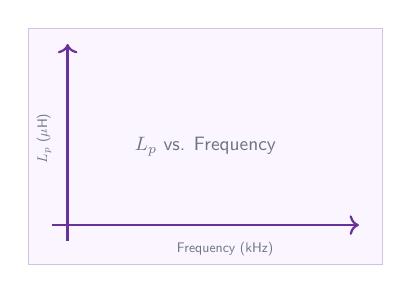
\begin{tikzpicture}
    \draw[fill=lightbg, draw=primary!30] (0,0) rectangle (45mm, 30mm);
    \draw[primary, thick, ->] (3mm, 5mm) -- (42mm, 5mm);
    \draw[primary, thick, ->] (5mm, 3mm) -- (5mm, 28mm);
    \node[text=textmuted, scale=0.7] at (22.5mm, 15mm) {$L_p$ vs. Frequency};
    \node[text=textmuted, scale=0.5] at (25mm, 2mm) {Frequency (kHz)};
    \node[text=textmuted, scale=0.5, rotate=90] at (2mm, 16mm) {$L_p$ ($\mu$H)};
\end{tikzpicture}
\end{minipage}
\hfill
\begin{minipage}[t]{0.32\textwidth}
\centering
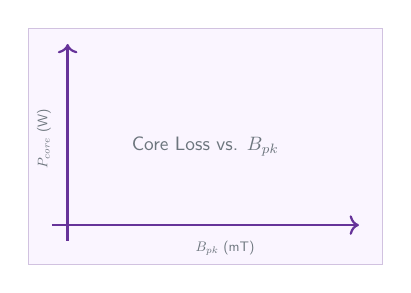
\begin{tikzpicture}
    \draw[fill=lightbg, draw=primary!30] (0,0) rectangle (45mm, 30mm);
    \draw[primary, thick, ->] (3mm, 5mm) -- (42mm, 5mm);
    \draw[primary, thick, ->] (5mm, 3mm) -- (5mm, 28mm);
    \node[text=textmuted, scale=0.7] at (22.5mm, 15mm) {Core Loss vs. $B_{pk}$};
    \node[text=textmuted, scale=0.5] at (25mm, 2mm) {$B_{pk}$ (mT)};
    \node[text=textmuted, scale=0.5, rotate=90] at (2mm, 16mm) {$P_{core}$ (W)};
\end{tikzpicture}
\end{minipage}
\hfill
\begin{minipage}[t]{0.32\textwidth}
\centering
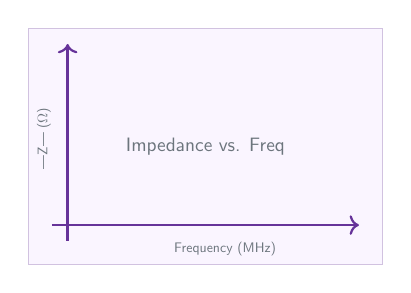
\begin{tikzpicture}
    \draw[fill=lightbg, draw=primary!30] (0,0) rectangle (45mm, 30mm);
    \draw[primary, thick, ->] (3mm, 5mm) -- (42mm, 5mm);
    \draw[primary, thick, ->] (5mm, 3mm) -- (5mm, 28mm);
    \node[text=textmuted, scale=0.7] at (22.5mm, 15mm) {Impedance vs. Freq};
    \node[text=textmuted, scale=0.5] at (25mm, 2mm) {Frequency (MHz)};
    \node[text=textmuted, scale=0.5, rotate=90] at (2mm, 16mm) {|Z| ($\Omega$)};
\end{tikzpicture}
\end{minipage}

\vspace{4mm}

% ═══════════════════════════════════════════════════════════════════════════════
% ENVIRONMENTAL & COMPLIANCE
% ═══════════════════════════════════════════════════════════════════════════════
\begin{minipage}[t]{0.48\textwidth}
\sectiontitle{Environmental Specifications}
{\footnotesize
\begin{tabular}{|L{35mm}|L{25mm}|}
\hline
\rowcolor{primary}
\textcolor{white}{\textbf{Parameter}} & \textcolor{white}{\textbf{Specification}} \\
\hline
Operating Temperature & -40 to +130°C \\
\rowcolor{gridbg}
Storage Temperature & -40 to +150°C \\
Humidity & 95\% RH max \\
\rowcolor{gridbg}
Altitude & Up to 5000m \\
\hline
\end{tabular}
}
\end{minipage}
\hfill
\begin{minipage}[t]{0.48\textwidth}
\sectiontitle{Compliance \& Certifications}
\begin{itemize}[leftmargin=4mm, itemsep=0pt, topsep=0pt]
    \item[\textcolor{success}{\checkmark}] RoHS 2015/863/EU Compliant
    \item[\textcolor{success}{\checkmark}] REACH SVHC Compliant
    \item[\textcolor{success}{\checkmark}] IEC 61558-2-16 Safety
    \item[\textcolor{success}{\checkmark}] UL/CSA Recognized
    \item[\textcolor{success}{\checkmark}] VDE Certified
\end{itemize}
\end{minipage}

\vspace{4mm}

% ═══════════════════════════════════════════════════════════════════════════════
% DIMENSIONS
% ═══════════════════════════════════════════════════════════════════════════════
\sectiontitle{Package Dimensions}

\begin{minipage}[t]{0.55\textwidth}
\centering
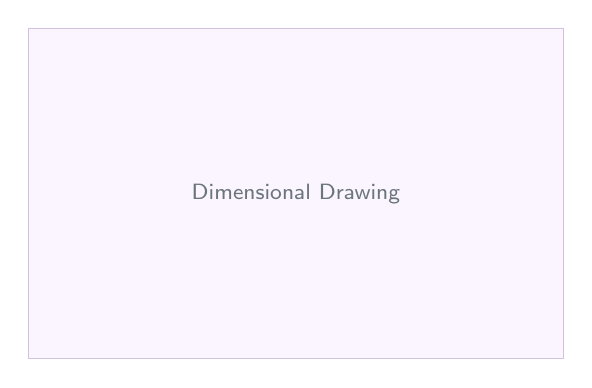
\begin{tikzpicture}
    \draw[fill=lightbg, draw=primary!30] (0,0) rectangle (68mm, 42mm);
    \node[text=textmuted] at (34mm, 21mm) {\footnotesize Dimensional Drawing};
\end{tikzpicture}
\end{minipage}
\hfill
\begin{minipage}[t]{0.42\textwidth}
{\footnotesize
\begin{tabular}{|L{20mm}|C{15mm}|C{12mm}|}
\hline
\rowcolor{primary}
\textcolor{white}{\textbf{Dimension}} & \textcolor{white}{\textbf{Value}} & \textcolor{white}{\textbf{Tol.}} \\
\hline
Length (A) & TBD & $\pm$0.5 \\
\rowcolor{gridbg}
Width (B) & TBD & $\pm$0.5 \\
Height (C) & TBD & $\pm$1.0 \\
\rowcolor{gridbg}
Pin Spacing & TBD & $\pm$0.3 \\
Weight & TBD g & - \\
\hline
\end{tabular}
}

\vspace{2mm}
{\footnotesize\color{textmuted} All dimensions in mm.}
\end{minipage}

\vspace{4mm}

% ═══════════════════════════════════════════════════════════════════════════════
% ORDERING INFORMATION
% ═══════════════════════════════════════════════════════════════════════════════
\sectiontitle{Ordering Information}

{\footnotesize
\begin{tabular}{|L{35mm}|C{20mm}|C{20mm}|C{25mm}|C{20mm}|C{20mm}|}
\hline
\rowcolor{primary}
\textcolor{white}{\textbf{Part Number}} & 
\textcolor{white}{\textbf{Turns Ratio}} & 
\textcolor{white}{\textbf{$L_p$ ($\mu$H)}} & 
\textcolor{white}{\textbf{Packaging}} & 
\textcolor{white}{\textbf{MOQ}} &
\textcolor{white}{\textbf{Lead Time}} \\
\hline
{{PART_NUMBER}} & {{TURNS_RATIO}} & {{MAGNETIZING_INDUCTANCE_UH}} & Tray / Bulk & 50 & 4-6 weeks \\
\hline
\end{tabular}
}

\vspace{3mm}

% ═══════════════════════════════════════════════════════════════════════════════
% FOOTER NOTES
% ═══════════════════════════════════════════════════════════════════════════════
\begin{tcolorbox}[
    colback=warning!10,
    colframe=warning!50,
    boxrule=0.3pt,
    arc=1mm,
    left=3mm,
    right=3mm,
    top=2mm,
    bottom=2mm
]
{\footnotesize\color{textdark}
\textbf{Important Notice:} Specifications subject to change without notice. Primary inductance measured at 1 kHz, 0.1 Vrms with secondary open. Leakage inductance measured with secondary shorted. For custom designs or modified specifications, contact {{COMPANY_NAME}} engineering.
}
\end{tcolorbox}

\vspace{2mm}
{\footnotesize\color{textmuted}
\textbf{Document History:} Rev. {{REVISION}} | Created: \today | Generated by OpenMagnetics
}

\label{LastPage}
\end{document}
